\newpage
\section{Materials \& Methods}

The session is divided into two parts, one checking if the air inside the apparatus can be considered ideal and one simulating a thermodynamic cycle. However, the main setup will be similar, with the equipment taken from the PASCO product TD-8572A, found at \cite{PASCO2024CavMan}.

\begin{wrapfigure}{r}{0.35\textwidth}  % 'r' for right, and width of 0.4 of the text width
    \centering
    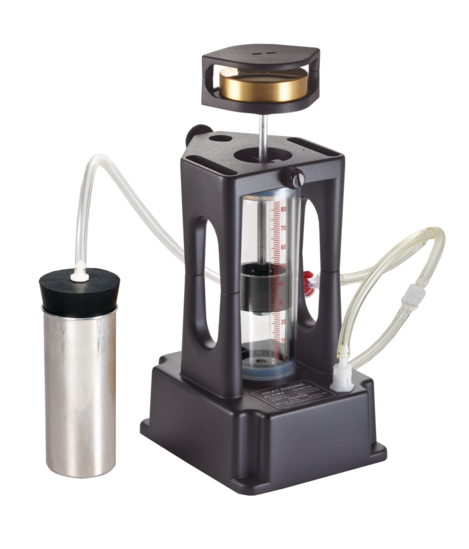
\includegraphics[width=0.35\textwidth]{Graphics/Apparatus.png}  % Adjust the width of the image
    \caption{Main apparatus of the heat engine, consisting of a thermal can connected to the Gas Law Apparatus. \cite{PASCO2024CavMan}}
    \label{fig:Apparatus}
\end{wrapfigure}

The main compartments of the heat engine were a metal thermal can and the Gas Law Apparatus. In the latter, a piston of radius $\mathit{r_p = (1.625 \pm 0.005)cm}$ could be found inside a glass cylinder with readings outside. The piston's movement could be controlled by either manually pushing the piston over a handle at the top, or screwing it at a fixed volume. If not fixed, the piston would smoothly increase the volume under higher pressures. Two ports for plastic tubes were available below the apparatus, both connected to the glass chamber. By connecting the metal can over plastic tubes to a Dual Pressure Sensor and one of these ports, air could only flow inside this system. The second port was also connected to the Dual Pressure Sensor to completely isolate the system. 

\begin{wrapfigure}{l}{0.4\textwidth}  % 'r' for right, and width of 0.4 of the text width
    \centering
    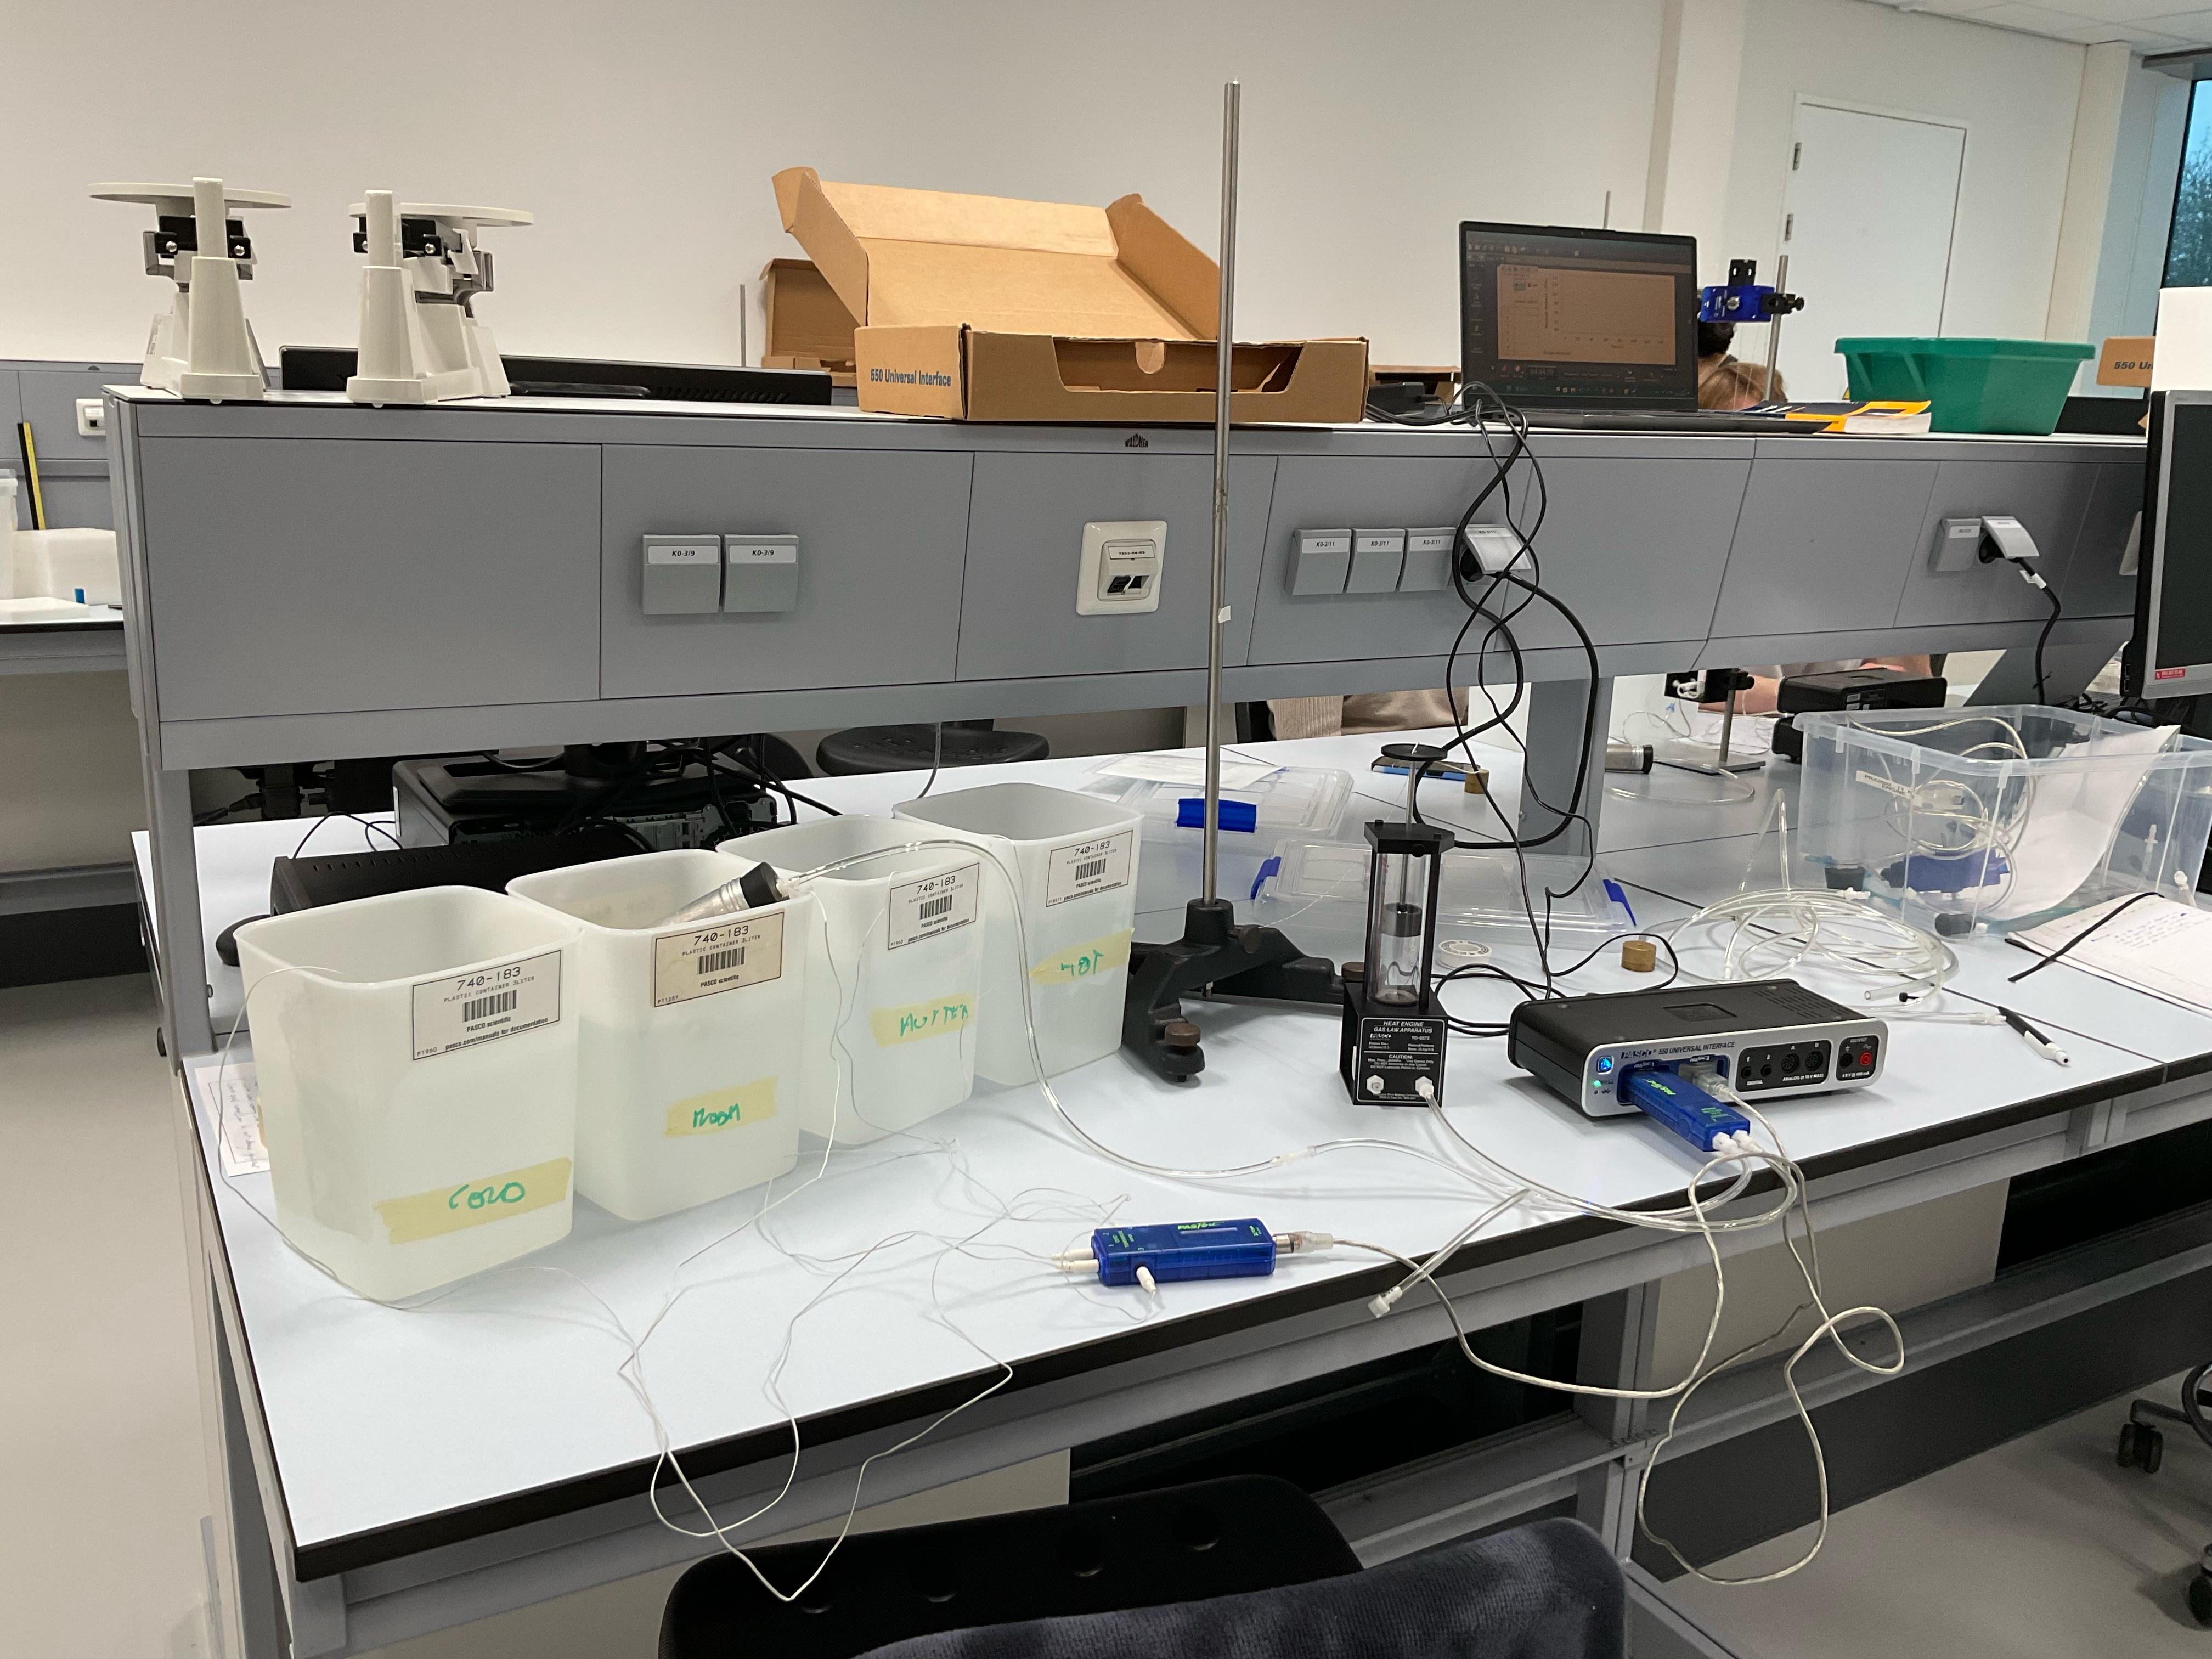
\includegraphics[width=0.35\textwidth]{Graphics/Ideal_Gas_Setup.jpeg}  % Adjust the width of the image
    \caption{Setup for ideal Gas Law Experiment. For comparison: The height of the metal rod inside the base is approx. 0.5m.}
    \label{fig:Ideal_Setup}
\end{wrapfigure}

For both experiments, the Dual Pressure Sensor and a Quad Temperature Sensor were connected over a PASCO Interface to PASCO Capstone, where the measurements could be quickly compiled. According to the producer, the device can read temperatures of all baths with an accuracy of approx. $\mathit{\pm 0.5 K}$.


\subsection{Evaluation Ideal Gas}
\label{Evaluation Ideal Gas}

To visualize the gas' ideality (i.e. how close its behaviour is to that of an ideal gas), the idea was to check one of the laws outlined in Section \ref{Ideal Gas Law}. It was decided to keep the volume constant and change the system's temperature, measuring the resultant pressure. An ideal gas would obey Gay-Lussac's Law (Equation \ref{eq:Gay-Lussac's Law}) and portray a positive linear correlation between pressure and temperature. As such, the piston was fixed over the screw.

Four thermal baths were prepared, each at vastly deviating temperatures. Fast Response Temperature Probes connected to the temperature sensor were placed in each container, with the readings documented in PASCO Capstone. 

Before conducting the measurements, a difficulty had to be addressed. At higher temperatures, the apparatus seemed to leak, meaning that over time the moles of gas $\mathit{n}$ would increase or decrease to adapt the system's pressure to its surroundings. Before each data logging, the apparatus was thus reset by unplugging the plastic tubes and placing the metal can inside a bath close to room temperature. The system was then isolated again, such that the can could be moved to the next reservoir. 

The data collected was used to plot a graph supposedly portraying the linear correlation between pressure $\mathit{P}$ and temperature $\mathit{T}$. 

\subsection{Simulating a Thermodynamic Cycle}
\label{Therm Cycle}

\begin{wrapfigure}{l}{0.4\textwidth}  % 'r' for right, and width of 0.4 of the text width
    \centering
    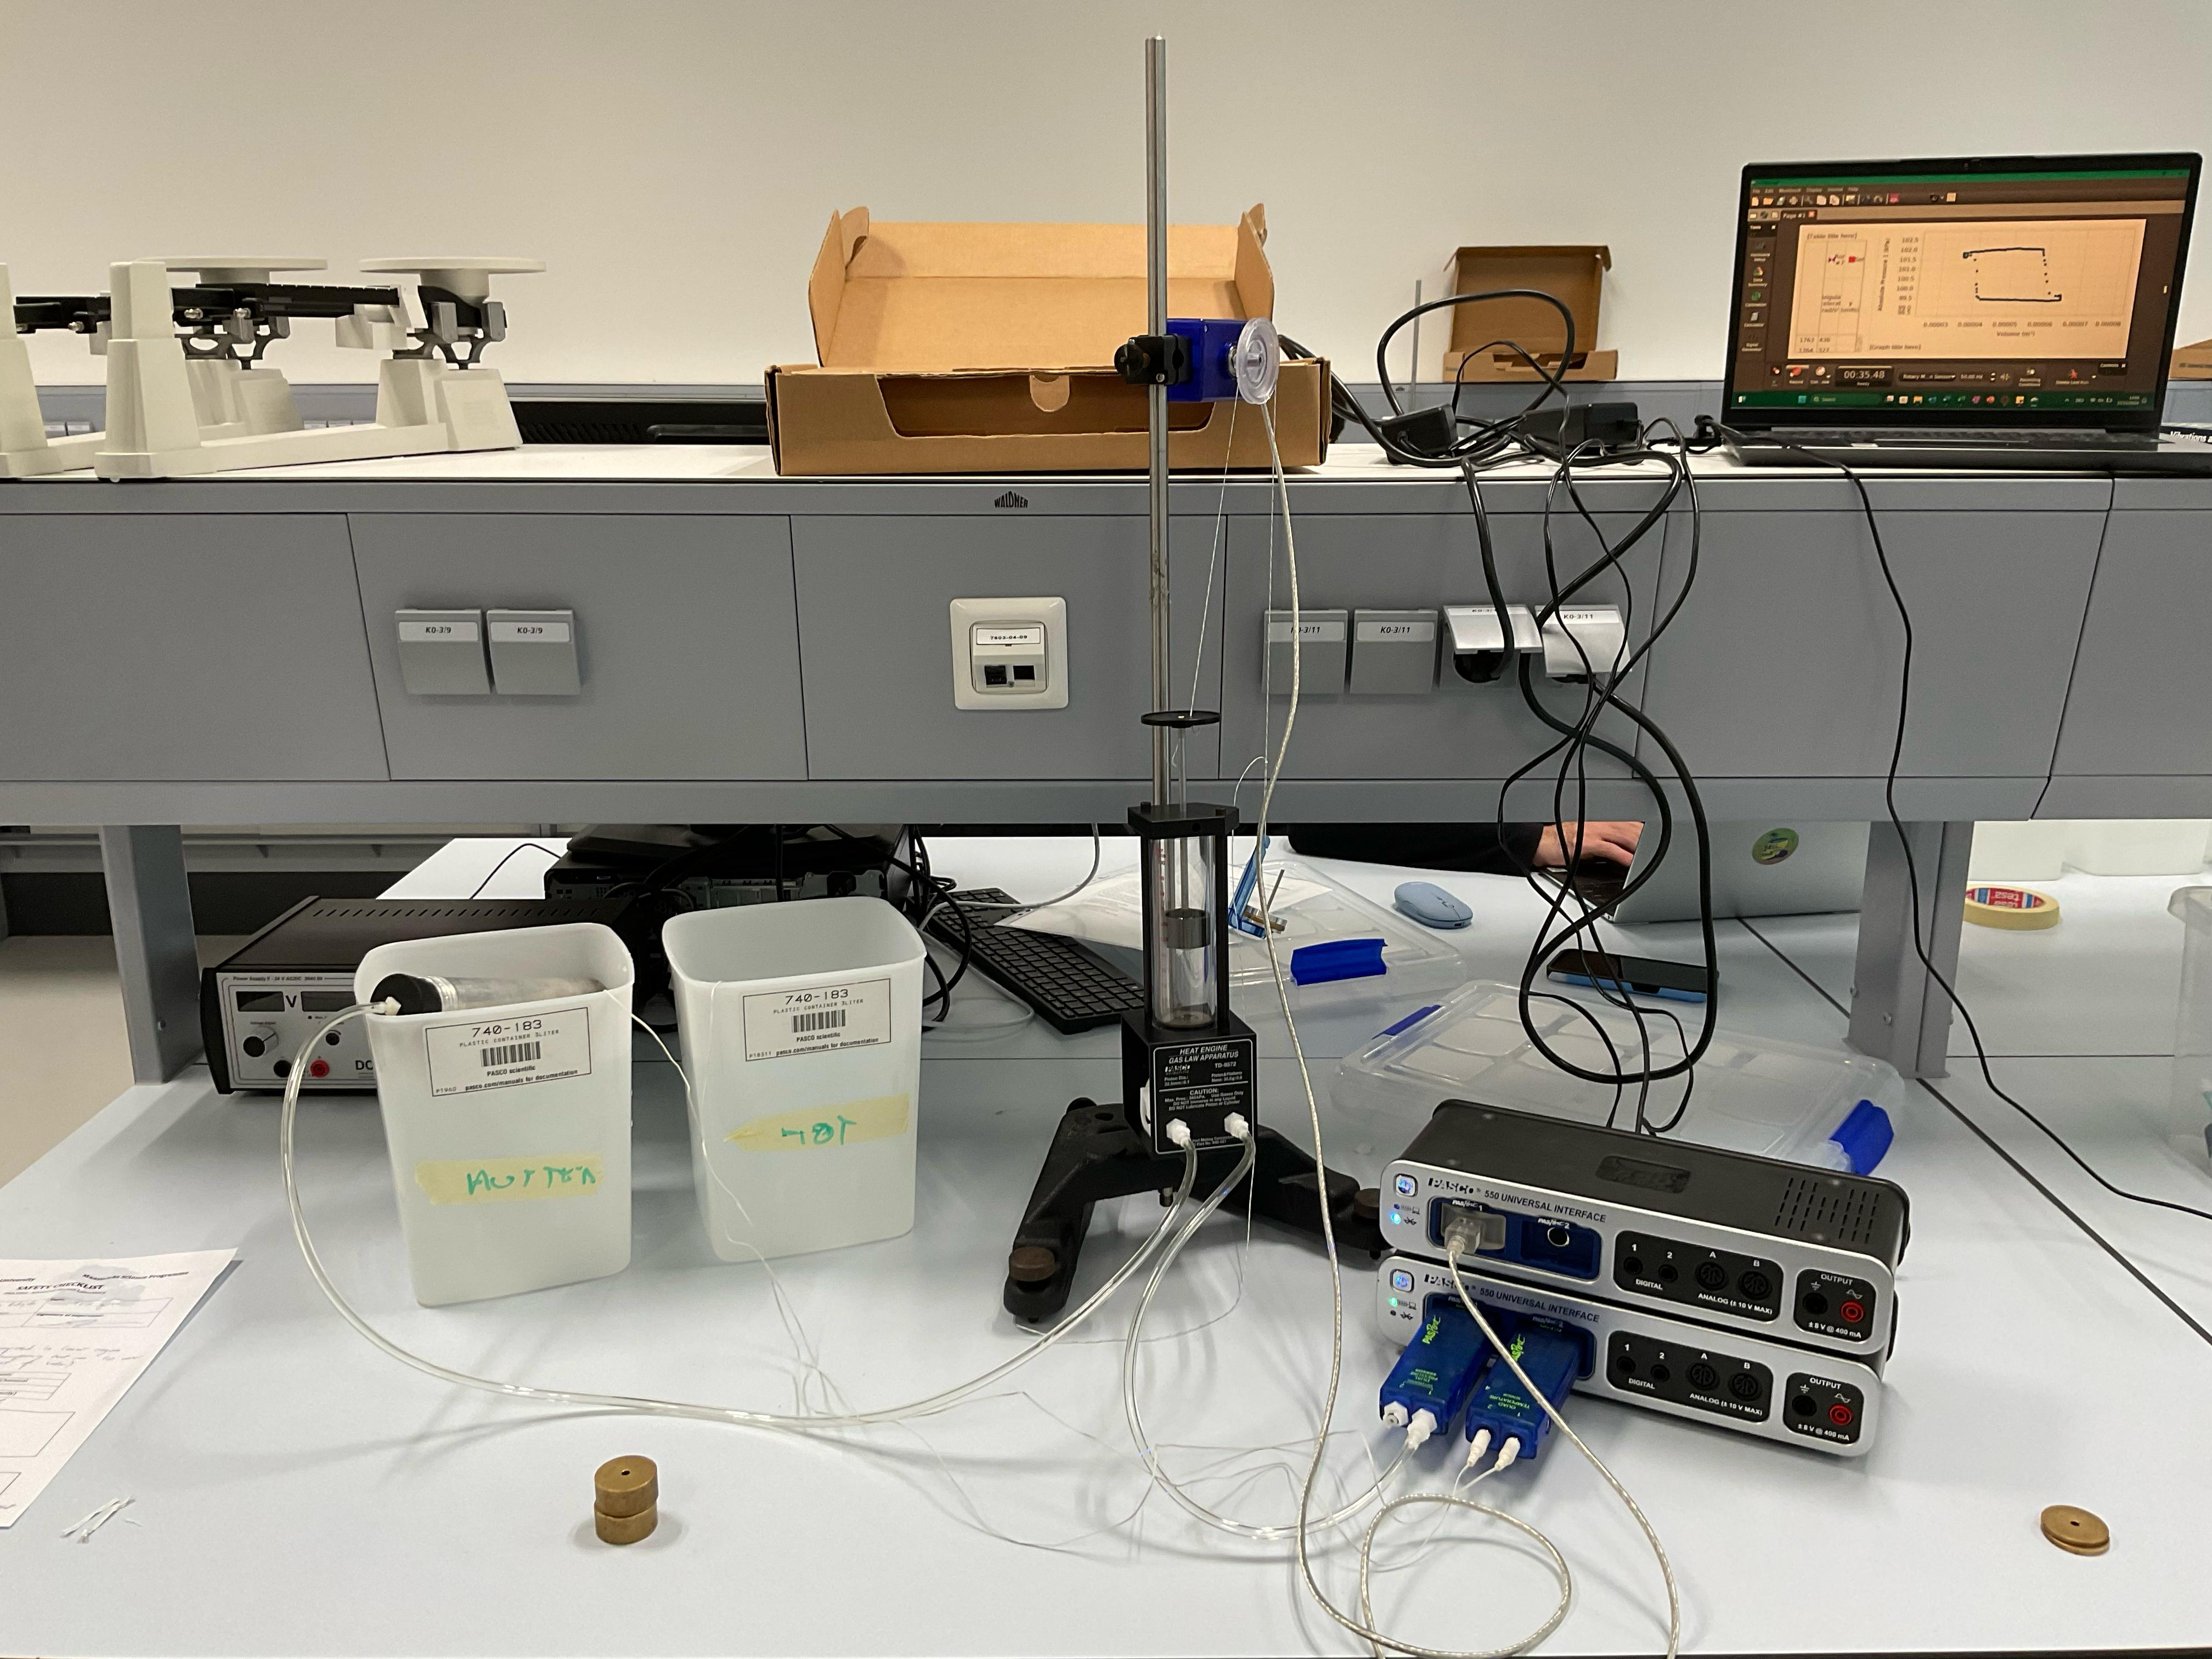
\includegraphics[width=0.35\textwidth]{Graphics/Cycle_Setup.jpeg}  % Adjust the width of the image
    \caption{Setup for Thermodynamic Cycle.}
    \label{fig:Cycle_Setup}
\end{wrapfigure}

The second part of the lab session considered the apparatus undergoing a thermodynamic cycle, closely resembling the Ericsson cycle. Two heat baths representing the hot and cold reservoirs were prepared, at temperatures vastly deviating from one another such that changes during thermodynamic processes could occur quickly. The temperatures were again measured through probes. 

The cycle consisted of four distinct processes, for which the setup had to be slightly altered. To begin with, the screw fixing the piston was removed in order to allow volumetric changes, which were assessed by a Rotary Motion Sensor. 

\begin{wrapfigure}{r}{0.35\textwidth}  % 'r' for right, and width of 0.4 of the text width
    \centering
    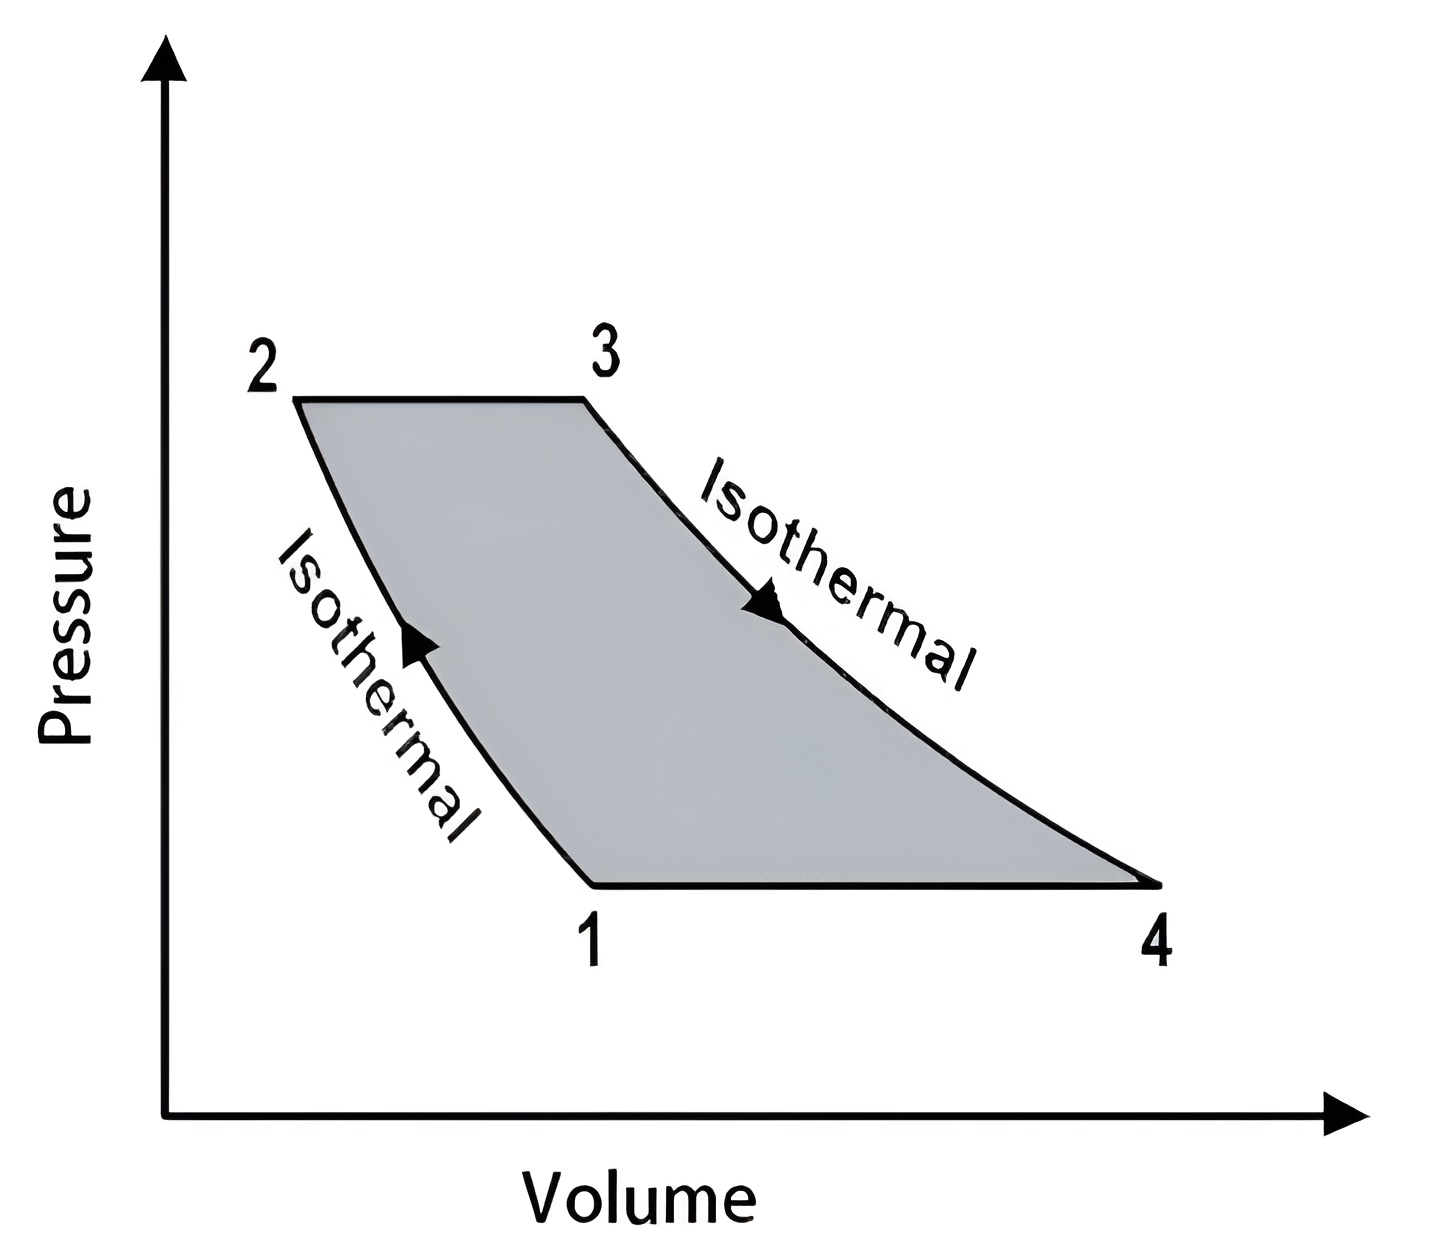
\includegraphics[width=0.45\textwidth]{Graphics/Ericsson_Cycle.png}  % Adjust the width of the image
    \caption{PV-Diagram of Ericsson Cycle: Two isothermal, two isobaric processes.}
    \label{fig:Ericsson Cycle}
\end{wrapfigure}

To counteract the weight of the piston pulling it down, equal masses were attached to it over a pulley. One could thus move the piston to a known initial position $\mathit{y_0}$ and leave it unperturbed. Although its position was originally set at $\mathit{y_0} = 0.05 m$, it was later realized that initial position had been altered during the several cycles in both directions by about $\mathit{\varepsilon_{y_0}= 0.003m}$. $\mathit{y_0 = (0.05 \pm 0.003) m}$ will be used following onwards. 

Since the volume of the plastic pipes and the metal can were not appraised by this group, the corresponding values will be taken from the student group surrounding Ana Tejero: $\mathit{V_{can} = 191.25 cm^3}$ and $\mathit{V_{pipes} = 13.09 cm^3}$. The total volume of the system can thus be calculated by:

\begin{equation}
\label{eq:Volume}
    \mathit{V = V_{can} + V_{pipes} + \pi r_p^2 (y_0 + y)}
\end{equation}

Here, $\mathit{y}$ is the displacement from initial position as measured by the Rotary Motion Sensor. From the formula, it can be seen that the error on the volume becomes $\mathit{\varepsilon_V = \pi r_P^2 \varepsilon_{y_0} \approx 2.489 \cdot 10^{-6} cm^3}$. Unfortunately, no uncertainties on the other volume values are known.

The setup was first acclimatized to room temperature. After plugging the open plastic tube into the apparatus and thus isolating the system, the can was placed in the cold reservoir and a PV-diagram was created. 

\textbf{Step I} will be thought of as displaying an isothermal compression, where a mass with $\mathit{m = 200g}$ was placed on top of the piston. However, later contemplations found in Section \ref{Thermodynamic Cycle Discussion} will contradict this approximation.

Next, in the isobaric expansion of \textbf{step II}, the metal can was moved to the hot reservoir and left there until the volume stopped increasing, meaning that equilibrium had been reached. 

After removing the mass (\textbf{step III}) and initiating an isothermal compression, the thermal can was inserted into the cold reservoir (\textbf{step IV}), a process of isobaric compression. 

The measurement was stopped when the PV-curve reached its original position.

Even though the process was repeated several times, only data from the first cycle will be analyzed, due to the error in the initial position being the lowest.

\subsubsection{Determining the Efficiency}
\label{Determining the Efficiency}

Over the temperatures of the cold and hot reservoirs measured at the beginning of each cycle, one could apply Equation \ref{eq:Carnot_Efficiency} to find the Carnot efficiency. Here, $\mathit{T_h = T_2 = T_3}$ and $\mathit{T_c = T_1 = T_4}$

Using Equation \ref{eq:Efficiency}, it is possible to calculate the engine's actual efficiency. The simplest method is to assess the area enclosed by the graphs in the PV-diagram, yielding the total work $\mathit{W}$ done per cycle. Additionally, by analyzing the type of thermodynamic process during each step, one can identify those where heat $\mathit{Q_h}$ was added to the system. 

In the described process, this would refer to the isobaric expansion in step II and the isothermal expansion in step III. Step III occurs at constant temperature, meaning that the internal energy is not affected: $\mathit{\Delta U_{III} = 0}$. From the Ideal Gas Law, it is found that $\mathit{P_3 V_3 = P_4 V_4 = const}$ during the process. The First Law of Thermodynamics can therefore be simplified:

\begin{equation}
\label{eq:Q_III}
    \mathit{Q_{III} = W_{III} = \int_{V_3}^{V_4} PdV = \int_{V_3}^{V_4} \frac{nRT}{V}dV = P_4 V_4 \ln{\frac{V_4}{V_3}}}
\end{equation}

At the end, $\mathit{P_4}$ and $\mathit{V_4}$ are chosen for convenience. 

Step II happens at constant pressure. 
The system the experiment centers around contains air, for which the composition is dominated by diatomic gases. Due to the degrees of freedom, the values for the specific heat capacities are given by $\mathit{C_V = \frac{5}{2}R}$ and $\mathit{C_P = \frac{7}{2}R}$. Equation \ref{eq:C_P} can be applied therefore:

\begin{equation}
\label{eq:Q_II}
    \mathit{Q_{II} = \frac{7}{2}nR \Delta T = \frac{7}{2} \frac{P_3 V_3}{T_h} (T_h-T_c) = \frac{7}{2} \frac{P_4 V_4}{T_h} (T_h-T_c)}
\end{equation}

The total heat absorbed is a combination of these two processes: $\mathit{Q_h = Q_{II} + Q_{III}}$.
The efficiency can be calculated from work $\mathit{W}$ and $\mathit{Q_h}$ alone.